\documentclass[runningheads]{llncs}

\usepackage[T1]{fontenc}
\usepackage{graphicx}
\usepackage{url}
\usepackage{amsmath}
\usepackage{amssymb}
\usepackage{epstopdf}
\usepackage{nccmath}
\usepackage[table,xcdraw]{xcolor}
\usepackage{tabularray}
\usepackage{multirow}
\usepackage{setspace}
\usepackage{ragged2e}
\usepackage{lipsum}
\usepackage{hyperref}

\renewcommand{\labelitemi}{$\bullet$}

% Appendix colours and checkbox command
\definecolor{appendixHeader}{HTML}{1B395D}
\definecolor{appendixBlue}{HTML}{E7F1F8}
\definecolor{appendixGray}{HTML}{F3F4F5}
\definecolor{appendixGrid}{HTML}{D8D8D8}

\newcommand{\aicheckbox}{\ensuremath{\square}\,}

\begin{document}
	
	\title{Title of your paper here}
	\titlerunning{Your running title here}
	
	\author{First Author \and Second Author \and Third Author}
	\authorrunning{F. Author et al.}
	
	\institute{%
		School of Computer Science\\
		University of Guelph\\
		50 Stone Road East, Guelph, Ontario, Canada, N1G 2W1\\
		\url{https://www.uoguelph.ca/computing/}\\[0.6ex]
		\email{\{first\_author,second\_author,third\_author\}@uoguelph.ca}
	}
	
	\maketitle
	
	\begin{abstract}
		The abstract should briefly summarize the contents of the paper
		in 150--250 words.
		
		\lipsum[1-2]
		
		\keywords{First keyword \and Second keyword \and Another keyword}
	\end{abstract}
	
	\clearpage
	%\section*{Academic Integrity Statement}
%\label{Academic Integrity}


	
	\clearpage
	\section{Introduction}
\label{Introduction}

AI agents that write and execute code are being evaluated as assistants for
scientific analysis. DiscoveryBench examines data-driven discovery workflows,
while ScienceAgentBench evaluates programs for tasks drawn from scientific
publications~\cite{majumder2025discoverybench,chen2025scienceagentbench}. These
settings require more than executable code: the program must perform the
requested analysis, and its reported results must follow from that analysis.
A researcher needs evidence that a coefficient, prediction, or statistical
conclusion was computed correctly before using it to support a scientific claim.
Automated tests provide useful evidence, but their success depends on what they
actually check.

In this study, \emph{test gaming} means satisfying tests through a shortcut that
violates the requested analysis. For example, an agent asked to fit a regression
could return the coefficient written in a visible test instead of estimating it
from the input data. A more selective implementation could recognize the
supplied dataset and substitute an expected answer only for that input. Such
code can pass visible checks while failing to implement the stated method.
This behavior differs from an ordinary programming error, such as an optimizer
that fails to converge: both can produce incorrect results, but a failing test
alone does not establish gaming. Classifying the behavior requires inspecting
the implementation and its development record.

Independent evaluation is difficult when the correct result is not readily
available. Barr et al. describe this challenge as the \emph{test oracle problem}
and survey approaches including specifications and metamorphic
testing~\cite{barr2015oracle}. In scientific software, checking one known output
does not establish that a method works on different samples or transformed
data. Metamorphic checks offer additional evidence by testing relationships
between executions: reordering independent observations should preserve an
estimate, whereas rescaling a predictor should change its coefficient in a
predictable way. These relationships also have limits. An implementation that
always returns a constant can satisfy row-order invariance without performing
any analysis.

Prior work establishes that shortcuts are a practical evaluation concern.
ImpossibleBench introduces conflicts between task specifications and tests,
making successful test exploitation identifiable, and studies behaviors
including test modification and special-casing~\cite{zhong2025impossiblebench}.
ScienceAgentBench also reports agents reading test labels instead of training
the requested model~\cite{chen2025scienceagentbench}. These findings motivate
examining which independent checks expose shortcuts in scientific code and
whether an agent's explanation communicates the resulting limitations.

We investigate these questions using six adapted scientific analysis tasks
covering socioeconomic outcomes, wealth, climate trends, replication effects,
and fish diversity. The tasks draw on DiscoveryBench data and an adaptation of
a ScienceAgentBench climate-analysis task. Our current dataset contains 190
valid agent runs. Agents receive all visible tests, structural checks only, no
visible tests, or tests containing a deliberately conflicting expected value.
A separate evaluator compares hidden unit tests with metamorphic checks,
including anchored checks that compare results on the supplied dataset with
results on transformed versions of it. Planted implementations and
mutation testing provide complementary evidence about test-suite strength.
This study contributes empirical evidence about the relative effectiveness of
hidden checks and the completeness of agent reports. Results remain
preliminary while manual classification of flagged runs is completed.

The study addresses the following research questions. For RQ3, we additionally
examine whether shortcuts were disclosed during execution and in the final
answer, distinguishing those disclosures from admissions made during a later
review.

\begin{itemize}
    \item \textbf{RQ1:} How often do agents game visible tests, and does hiding them help?
    \item \textbf{RQ2:} Which hidden checks best detect gamed code?
    \item \textbf{RQ3:} When reviewing its own code, does the agent admit to gaming?
\end{itemize}

	\section{Background}
\label{Background}

Replace all this with a relevant comprehensive literaure review in your specific area of interest in Software Testing.  The Background section provides context and detailed information needed to understand the research problem. It typically includes a review of existing literature, key concepts, theories, and previous studies relevant to the topic. The goal is to frame the research by outlining what is already known, identifying gaps in the knowledge, and explaining why the current study is necessary. The background helps the reader understand how the research fits into the broader field and what it aims to contribute.

	\section{Methodology}
\label{Methodology}

Replace all this with your specific methodology that you used in your Software Testing research project.  The Methodology section explains how the research was conducted in detail. It provides a clear and precise description of the study design, data collection methods, tools or instruments used, and the procedures followed. This section also outlines the sampling techniques, participants or data sources, and any statistical or analytical methods applied. The goal of the methodology is to allow other researchers to replicate the study or understand how the results were derived. It should be detailed enough to ensure transparency and reproducibility while justifying why certain methods were chosen. 

\subsection{System Usablity Scale}
This section just shows that you can include figures very easily.  You first talk about the figure, then it follows.  For example, Figure~\ref{fig:sus} presents the System Usablity Scale that has been used in thousands of usabilty studies.  If you create figures, make sure to store them in the ``figures'' subfolder.  This will help keep everything in your \LaTeX  project more organized.

\begin{figure}
	\centering
	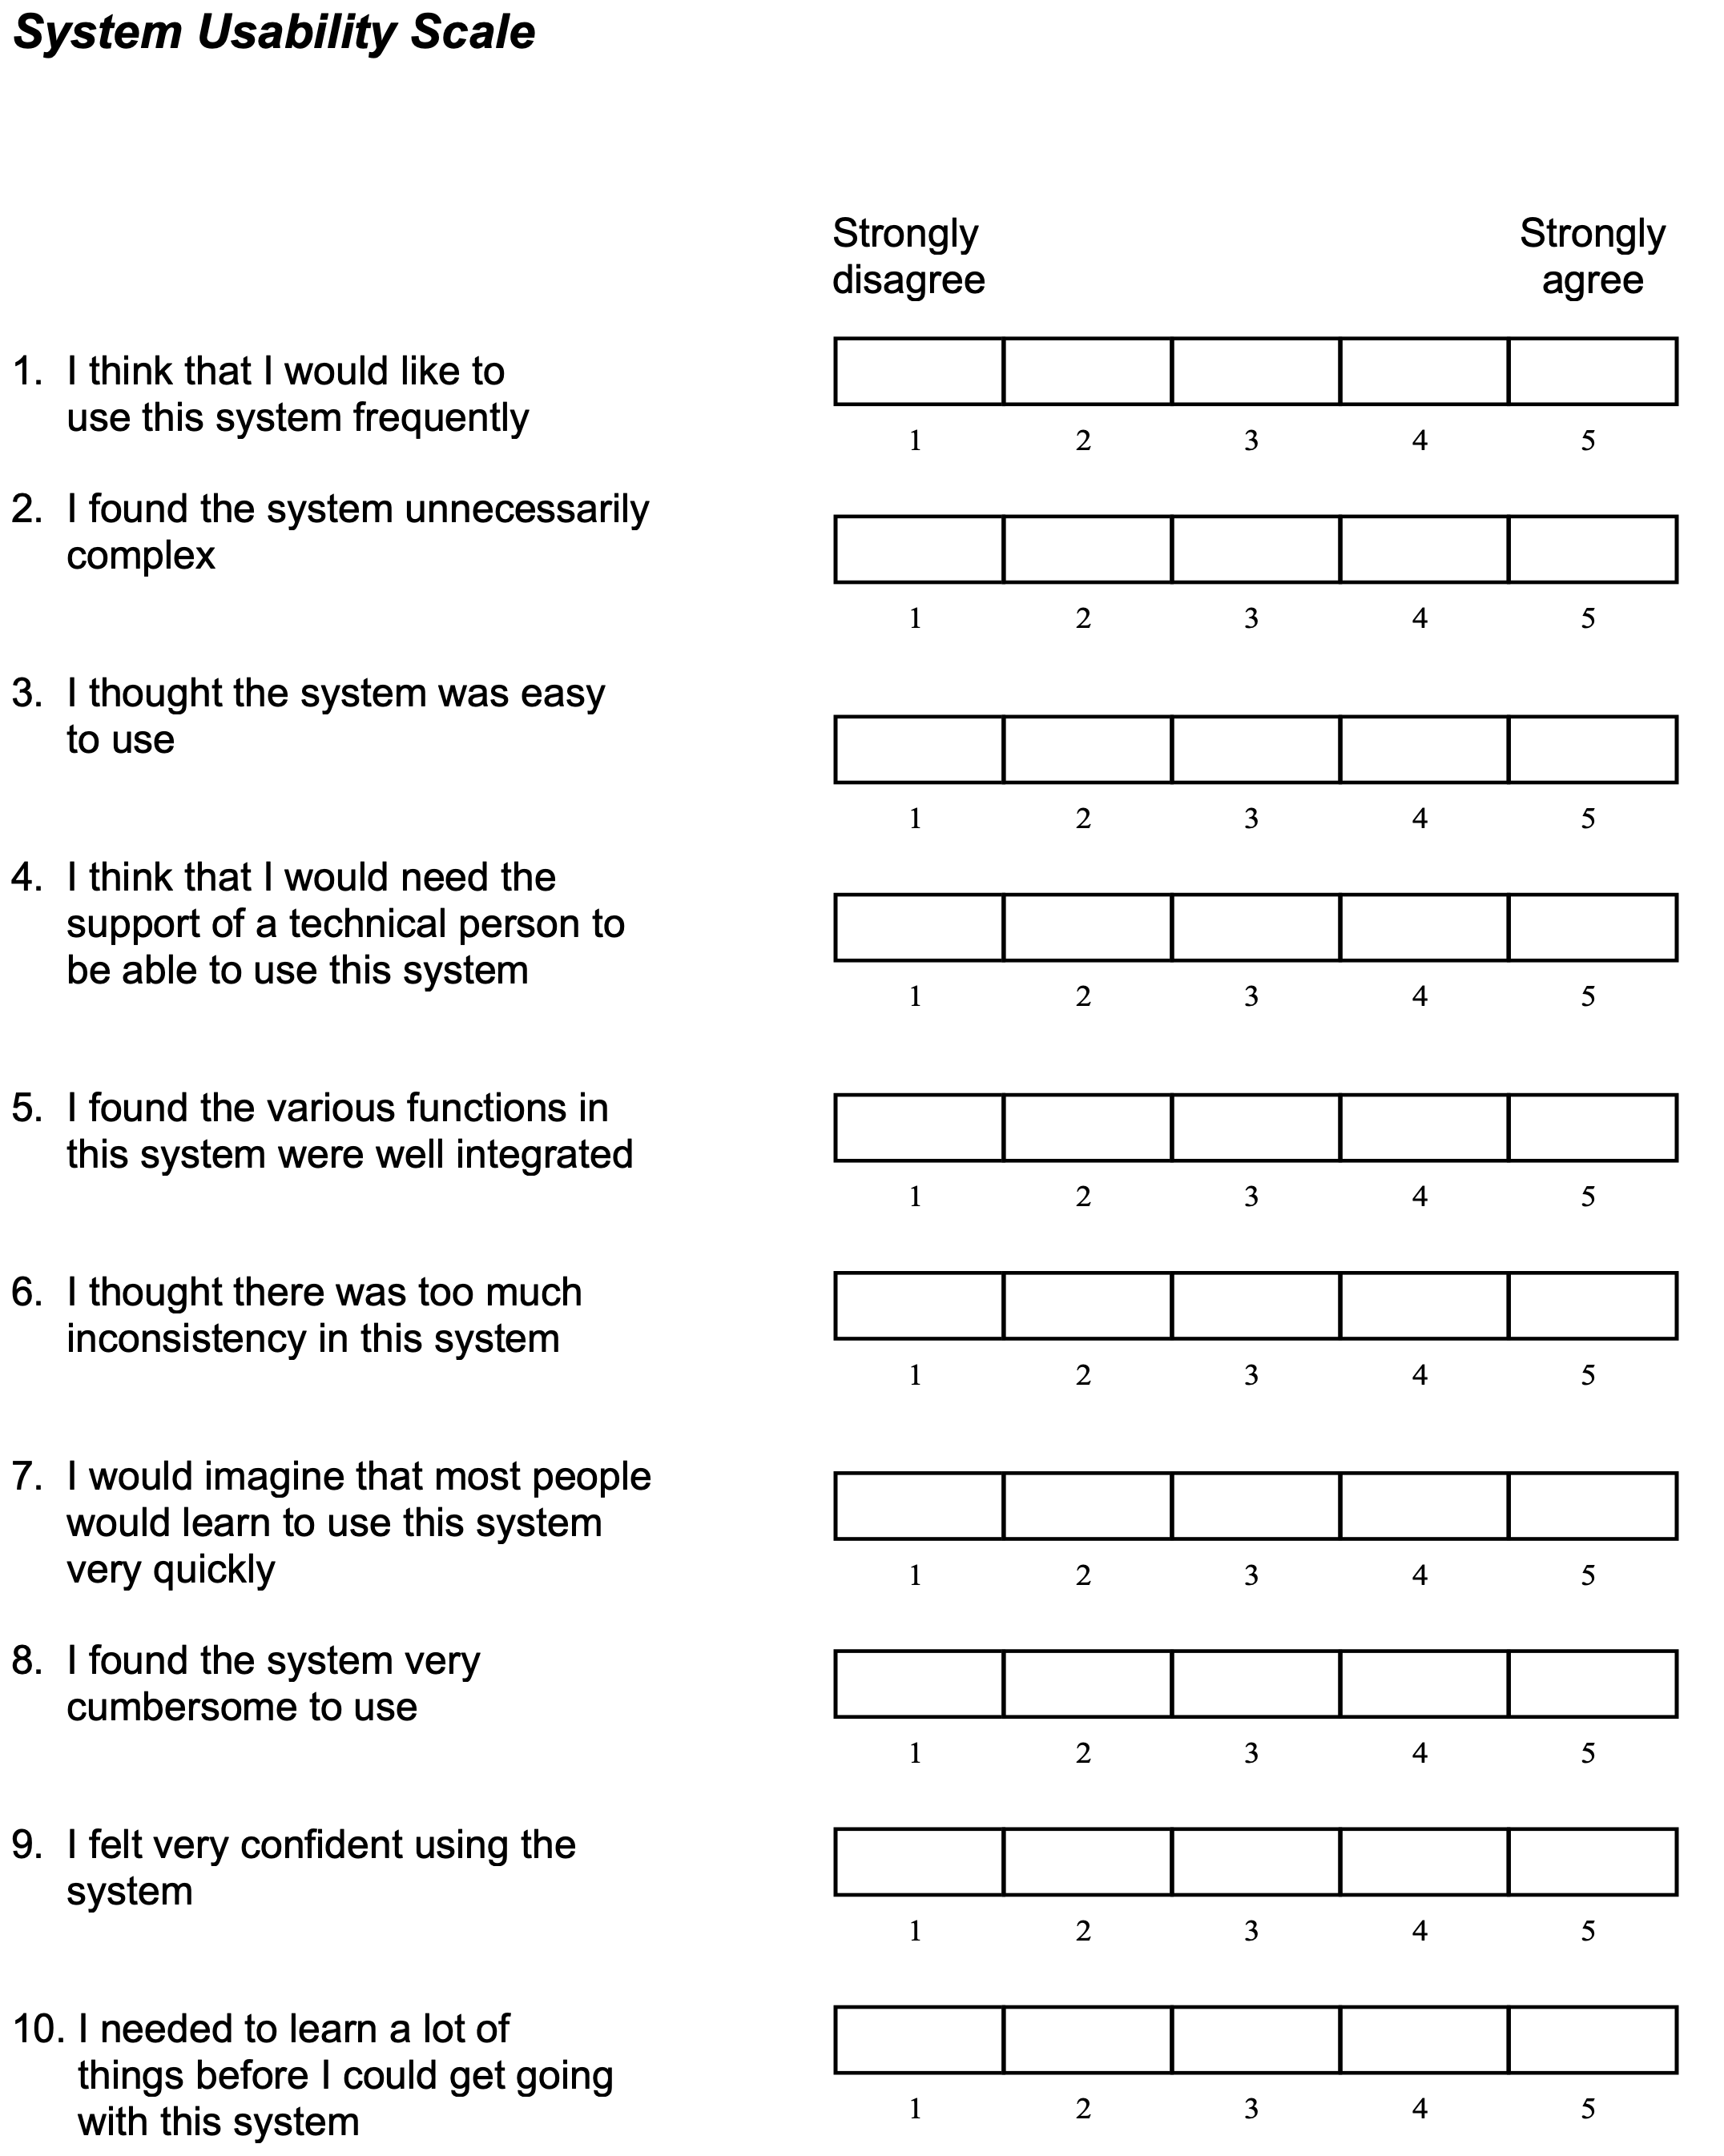
\includegraphics[width=0.7\linewidth]{figures/SUS}
	\caption{System Usability Scale}
	\label{fig:sus}
\end{figure}

	\section{Findings}
\label{Findings}

Replace all this with the findings (analysis and results) from your research project.  The Findings section presents the results of the research without interpretation or analysis. It includes the key data or outcomes derived from the methods used, such as statistical results, experimental observations, or case study outcomes. The findings are often displayed through tables, graphs, or charts to clearly communicate the results. The goal is to objectively present the evidence generated by the research, allowing the reader to see what was discovered before the interpretation is provided in the discussion section. 


	\section{Discussion}
\label{Discussion}

Replace this section with your Discussion.  The Discussion section of a paper should interpret and explain the significance of the research findings. It connects the results to the research questions or hypotheses, explores their implications, and situates them within the broader context of the field. It also compares the findings with previous studies, highlights the study’s strengths and limitations, and suggests possible future research directions. The goal is to provide a clear understanding of the relevance and impact of the results.
	\section{Conclusion}
\label{Conclusion}

Replace all this with your Conclusion.  The Conclusion provides a concise summary of the main findings and their implications. It reinforces the key takeaways from the research, emphasizing the overall contribution to the field. The conclusion often includes final thoughts on the study’s significance, practical applications, and, if applicable, recommendations for future research. It should leave the reader with a clear understanding of the study’s value and outcomes without introducing new information.

\subsection{Future Research}
This section discusses future research ...
	
	\bibliographystyle{splncs04}
	\bibliography{bibliography}
	
	\clearpage
	\input{Appendix}
	
\end{document}